\section{Min-Max Optimization}

The min-max problem is defined as $\min_{x\in X} \max_{y \in Y} \phi(x,y)$.

\textbf{Definitions}:
\begin{enumerate}
    \item \textbf{Saddle point and minimax point}: $(x^*, y^*)$ is a saddle point if $\phi(x^*, y) \le \phi(x^*, y^*) \le \phi(x, y^*)$ for any $x, y$. $(x^*, y^*)$ is a global minimax point if $\phi(x^*, y) \le \phi(x^*, y^*) \le \max_{y^\prime \in Y} \phi(x, y^\prime)$ for any $x, y$. Game theory interpretation: saddle point means Nash equilibrium, where no play has the incentive to make unilateral changes; global minimax point is Stackelberg equilibrium, where it is the best response to the best response.
    \item \textbf{Convex-concave function}: $\phi(x, y)$ is convex-concave if $\phi(x, y)$ is convex for every fixed $y$ and $\phi(x,y)$ is concave for every fixed $x$.
    \item \textbf{Strongly-convex-strongly-concave function}: $\phi(x, y)$ is strongly-convex-strongly-concave if $\phi(x, y)$ is $\mu_1$-strongly convex for every fixed $y$ and $\phi(x,y)$ is $\mu_2$-strongly concave for every fixed $x$.
    \item \textbf{Smoothness jointly in $x$ and $y$}: $\|\nabla_x \phi(x_1, y_1) - \nabla_x \phi(x_2, y_2)\| \le L(\|x_1 - x_2\| + \|y_1 - y_2\|)$ and $\|\nabla_y \phi(x_1, y_1) - \nabla_y \phi(x_2, y_2)\| \le L(\|x_1 - x_2\| + \|y_1 - y_2\|)$.
    \item \textbf{Duality gap}: defined to be $\max_y \phi(\hat{x}, y) - \min_x \phi(x, \hat{y})$. When duality gap is smaller than or equal to $\epsilon$, we say $(\hat{x}, \hat{y})$ is an $\epsilon$-saddle point.
    \item \textbf{Monotone operators}: A operator $F$ is monotone if $(F(u) - F(v))^\top (u-v) \ge 0$ for any $u,v$; it is $\mu$-strongly monotone if $(F(u) - F(v))^\top (u-v) \ge \mu \|u-v\|^2$ for any $u,v$.
\end{enumerate}

\textbf{Properties}:
\begin{enumerate}
    \item \textbf{Characterization of saddle points}: Define $\bar{\phi}(x) = \max_y \phi(x,y)$ and $\underline{\phi}(y) = \min_x \phi(x,y)$. Then $(x^*, y^*)$ is a saddle point iff $\max_y \min_x \phi(x,y) = \min_x \max_y \phi(x,y)$, $x^* \in \argmin_x \bar{\phi(x)}$ and $y^* \in \argmax_y \underline{\phi}(y)$. Proof: by definition.
    \item \textbf{Minimax Theorem}: If $X$ and $Y$ are closed convex sets, one of them is bounded, and $\phi(x,y)$ is a continuous convex-concave function, then there exists a saddle point on $X \times Y$ and $\max_y \min_x \phi(x, y) = \min \max \phi(x, y)$.
\end{enumerate}

\textbf{Gradient Descent Ascent}: do $x_{t+1} = \Pi_X(x_t - \gamma \nabla_x \phi(x_t, y_t))$ and $y_{t+1} = \Pi_Y (y_t + \gamma \nabla_y \phi(x_t, y_t))$. This simultaneously updates $x$ and $y$.

\textbf{Analysis}:
\begin{enumerate}
    \item \textbf{SC-SC and smooth fucntions}: (12.5) with $\gamma = \frac{\mu}{4L^2}$, GDA converges linearly: $\|x_{t+1} - x^*\|^2 + \|y_{t+1} - y^*\|^2 \le (1-4\mu^2/L^2)(\|x_t - x^*\|^2 + \|y_t - y^*\|^2)$. Proof: by SC-SC, $(\nabla_x f(x,y) - \nabla_x f(x^*, y^*))^\top (x - x^*) + (\nabla_y f(x^*, y^*) - \nabla_y f(x,y))^\top (y-y^*) \ge \mu\|x - x^*\|^2 + \mu\|y-y^*\|^2$. By smoothness, $\|\nabla_x \phi(x_1, y_1) - \nabla_x \phi(x_2, y_2)\|^2 + \|\nabla_y \phi(x_1, y_1) - \nabla_y \phi(x_2, y_2)\|^2 \le 4L(\|x_1 - x_2\|^2 + \|y_1 - y_2\|^2)$. Using these in the update gives the result.
    \item \textbf{C-C functions}: may not converge, e.g. $\phi(x,y) = xy$. Proof: $x_{t+1}^2 + y_{t+1}^2 = (x_t - \gamma y_t)^2 + (y_t + \gamma x_t)^2 = (1+\gamma^2)(x_t^2 + y_t^2)$.
\end{enumerate}

\textbf{Extragradient Method}: 

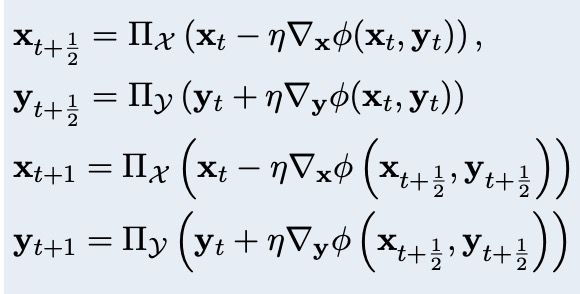
\includegraphics[width=\linewidth]{imgs/EG.jpg}

This is different from two steps of GDA, because the second step still uses the value of $t$. Essentially, EG is to use better gradients than GDA. EG has $O(1/T)$ convergece rate of the duality gap for averaged $x_{t+1/2}$ and $y_{t+1/2}$ in the C-C setting with bounded domain, and $O(\log(\frac{1}{\epsilon}))$ complexity in the SC-SC setting, which is optimal.

\textbf{Optimistic GDA}

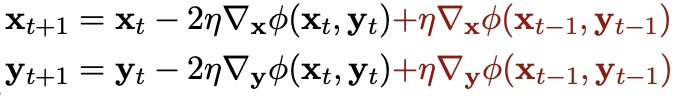
\includegraphics[width=\linewidth]{imgs/OGDA.jpg}

This is equivalent to:

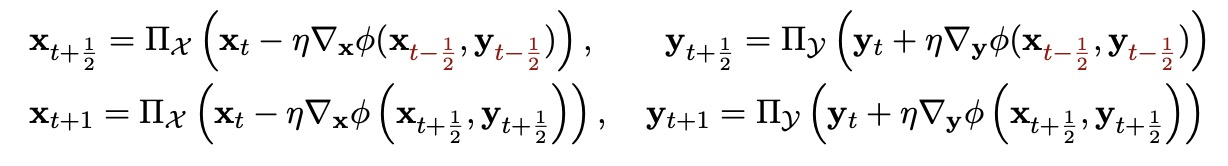
\includegraphics[width=\linewidth]{imgs/OGDA2.jpg}

OGDA has similar convergence rate as EG in the SC-SC and C-C settings.

\textbf{Proximal Point Algorithm}

do $(x_{t+1}, y_{t+1}) = \argmin_x \argmax_y \{\phi(x,y) + \frac{1}{2\eta} \|x-x_t\|^2 - \frac{1}{2\eta} \|y - y_t\|^2\}$.

This is equivalent to

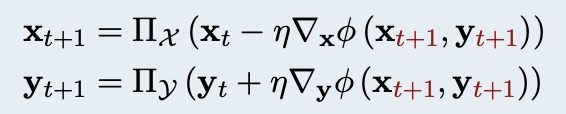
\includegraphics[width=\linewidth]{imgs/PPA.jpg}

PPA converges with $O(1/T)$ in the C-C setting. PPA, EG, OGDA and GDA are all using some estimation of the gradient.

\textbf{Concave games}: finite number of players $\mathcal{N} = \{1,\dots,N\}$, compact convex action set $X_i$, the utility function $u_i(x_i, x_{-i})$ is concave in $x_i$ for all $x_{-i}$.

\textbf{Nash equilibrium for concave games}: $u_i(x^*_i, x^*_{-i}) \ge u_i(x_i, x^*_{-i})$ for any $x_i \in X_i$. First-order characterization: in the concave game, Nash equilibria can be characterized as $\nabla_i u_i(x^*_i, x^*_{-i})^\top (x_i-x^*_i) \le 0$.

\textbf{Variational inequality problem}: find $z^* \in Z$ such that $F(z^*)^\top (z-z^*) \ge 0$ for all $z \in Z$. Existence: If $Z$ is a nonempty convex compact set and $F$ is continuous, then VI has a solution.

\textbf{Strong and weak solution of VI}: $z^*$ is a strong solution if $F(z^*)^\top (z-z^*) \ge 0$ for any $z$; $z^*$ is a weak solution if $F(z)^\top (z-z^*) \ge 0$. If $F$ is monotone, then a strong solution is a weak solution; If $F$ is continuous, then a weak solution is a strong solution.

\textbf{Min-max is a special case of VI}: let $F = (\nabla_x \phi, -\nabla_y \phi(y))$ makes it a VI. A point is a solution to this VI iff it is a saddle point.

\textbf{Solving VI by EG}: assume $Z$ is a closed convex set, the VI problem has solutions, $F$ is monotone and $L$-Lipschitz continuous, then EG: $\tilde{z_{t+1}} = \Pi_Z(z_t - \eta_t F(z_t))$ and $z_{t+1} = \Pi_Z(z_t - \eta_t F(\tilde(z)_{t+1}))$ converges in $O(1/T)$.